\documentclass[12pt, a4paper]{article}

% ── Packages ──────────────────────────────────────────────────────────────────
\usepackage[a4paper, margin=2.5cm]{geometry}
\usepackage{graphicx}
\usepackage{float}
\usepackage{amsmath}
\usepackage{amssymb}
\usepackage{xcolor}
\usepackage{mdframed}
\usepackage{parskip}
\usepackage{enumitem}
\usepackage{titlesec}
\usepackage{booktabs}
\usepackage{tikz}
\usepackage{hyperref}
\usepackage[T1]{fontenc}

% ── Graphics path ─────────────────────────────────────────────────────────────
\graphicspath{{../../Images_for_latex/Lecture_9/}}

% ── Colours ───────────────────────────────────────────────────────────────────
\definecolor{keyblue}{RGB}{30, 80, 160}
\definecolor{keybluebg}{RGB}{220, 235, 255}
\definecolor{noteorange}{RGB}{200, 100, 0}
\definecolor{noteorangebg}{RGB}{255, 240, 215}
\definecolor{warnred}{RGB}{180, 30, 30}
\definecolor{warnredbg}{RGB}{255, 220, 220}
\definecolor{defgreen}{RGB}{20, 110, 50}
\definecolor{defgreenbg}{RGB}{215, 245, 225}
\definecolor{headernavy}{RGB}{25, 35, 90}

% ── Box environments ──────────────────────────────────────────────────────────
\newmdenv[linecolor=keyblue,backgroundcolor=keybluebg,linewidth=1.5pt,
  leftline=true,rightline=false,topline=false,bottomline=false,
  innerleftmargin=10pt,innerrightmargin=8pt,
  innertopmargin=6pt,innerbottommargin=6pt,
  skipabove=8pt,skipbelow=8pt]{keybox}

\newmdenv[linecolor=noteorange,backgroundcolor=noteorangebg,linewidth=1.5pt,
  leftline=true,rightline=false,topline=false,bottomline=false,
  innerleftmargin=10pt,innerrightmargin=8pt,
  innertopmargin=6pt,innerbottommargin=6pt,
  skipabove=8pt,skipbelow=8pt]{notebox}

\newmdenv[linecolor=warnred,backgroundcolor=warnredbg,linewidth=1.5pt,
  leftline=true,rightline=false,topline=false,bottomline=false,
  innerleftmargin=10pt,innerrightmargin=8pt,
  innertopmargin=6pt,innerbottommargin=6pt,
  skipabove=8pt,skipbelow=8pt]{warnbox}

\newmdenv[linecolor=defgreen,backgroundcolor=defgreenbg,linewidth=1.5pt,
  leftline=true,rightline=false,topline=false,bottomline=false,
  innerleftmargin=10pt,innerrightmargin=8pt,
  innertopmargin=6pt,innerbottommargin=6pt,
  skipabove=8pt,skipbelow=8pt]{defbox}

% ── Section formatting ────────────────────────────────────────────────────────
\titleformat{\section}[block]{\large\bfseries\color{headernavy}}{}{0pt}{}
  [\vspace{2pt}\rule{\linewidth}{0.8pt}\vspace{4pt}]
\titleformat{\subsection}[block]{\normalsize\bfseries\color{keyblue}}{}{0pt}{}

% ── Document ──────────────────────────────────────────────────────────────────
\begin{document}

\begin{center}
  {\LARGE\bfseries\color{headernavy} Sensors \& Systems}\\[4pt]
  {\large Model Uncertainty and Validation}\\[2pt]
  {\normalsize Torben Knudsen \quad|\quad Electronic Systems, 8th Semester}
\end{center}

\vspace{4pt}\hrule height 1.2pt\vspace{12pt}

% ==============================================================================
\section*{Section 1 \quad Model Uncertainty}
% ==============================================================================

\begin{figure}[H]
  \centering
  
\includegraphics[width=0.78\textwidth]{slide-03.jpg}
  \caption{Overview of the approaches to dealing with model uncertainty.
    The lecture covers the first three; H-infinity filter design is an
    alternative that is not discussed further here.}
\end{figure}

Every model used in a Kalman filter, controller, or estimator is an
approximation of a real physical system.
In practice, some degree of \textbf{model uncertainty is unavoidable} ---
it arises from simplifications made during modelling, parameters that are
not precisely known, components that vary between units, or dynamics that
change over time.

The key question is not whether uncertainty exists, but \textbf{how to
handle it}.
There are four main strategies:

\begin{itemize}[leftmargin=1.5em, itemsep=5pt]

  \item \textbf{Model validation} --- test whether the current model is
    good enough for its intended purpose, and check statistically whether
    the residuals (prediction errors) look the way they should if the model
    were correct.
    If the model is wrong, this reveals it.
    \emph{Covered in Section~2.}

  \item \textbf{Multi-model estimation} --- when you cannot decide between
    several candidate models, run all of them in parallel and let the data
    determine which is most likely correct at each time step.
    The final state estimate is a probability-weighted combination of all
    model-specific estimates.
    \emph{Covered in Section~3.}

  \item \textbf{Estimating uncertain parameters} --- if the model structure
    is correct but some numerical parameters are unknown or slowly drifting,
    treat those parameters as extra states and estimate them alongside the
    physical states using an EKF/UKF, or use system identification methods
    (maximum likelihood) to find the best-fitting values offline.
    \emph{Covered in Section~4.}

  \item \textbf{H-infinity filter design} --- an alternative to the Kalman
    filter that does not assume Gaussian noise and instead minimises the
    worst-case estimation error.
    Robust to model uncertainty by design, but more conservative.
    \emph{Not covered further in this lecture.}

\end{itemize}

\begin{notebox}
  \textbf{Why model uncertainty always exists in practice}

  When building a state-space model $\dot{x} = f(x,u) + w$,
  $y = h(x) + v$, every design choice is an approximation:

  \begin{itemize}[leftmargin=1.5em, itemsep=2pt]
    \item \emph{Linearisation:} nonlinear systems are often approximated
      as linear around an operating point.
      Away from that point, the model is wrong.
    \item \emph{Unknown parameters:} spring stiffness, damping
      coefficients, friction --- these are rarely known exactly and vary
      between physical units of the same design.
    \item \emph{Changing dynamics:} a vehicle's mass changes as fuel is
      consumed; a robot arm's inertia changes as it picks up and puts down
      objects; a battery's internal resistance grows with age.
    \item \emph{Ignored dynamics:} real systems have resonances, delays,
      and nonlinearities that are deliberately left out of the model to
      keep it tractable.
      Those omitted effects still show up in the data.
  \end{itemize}

  None of these can be eliminated entirely.
  The three strategies in this lecture provide principled ways to detect,
  quantify, and compensate for these inevitable discrepancies.
\end{notebox}

% ── Key takeaways ─────────────────────────────────────────────────────────────
\begin{keybox}
  \textbf{Section 1 --- Key Takeaways}
  \begin{itemize}[leftmargin=1.2em, itemsep=2pt]
    \item Model uncertainty is unavoidable --- every model is an
      approximation.
      The question is how to detect and handle it.
    \item Three strategies are covered: \textbf{validation} (is the model
      good enough?), \textbf{multi-model estimation} (run competing
      models in parallel), and \textbf{parameter estimation} (estimate
      what you do not know).
    \item H-infinity design is a fourth robust alternative but not covered
      here.
  \end{itemize}
\end{keybox}

% ==============================================================================
\clearpage
\section*{Section 2 \quad Model Validation}
% ==============================================================================

Before applying a model to prediction, filtering, or control design, you
need to know whether it is fit for purpose.
Model validation provides two very different answers to two very different
questions.

\begin{notebox}
  \textbf{All three statistical tests use the same sequence}

  When the Kalman filter runs, it produces at every time step a
  \textbf{residual} (also called the innovation or output prediction
  error):
  \[
    \tilde{y}_{k|k-1} = y_k - \hat{y}_{k|k-1}
  \]
  This is simply the difference between what you actually measured
  ($y_k$) and what the model predicted you would measure
  ($\hat{y}_{k|k-1}$).
  After running the filter over your entire dataset you have a full
  sequence of these residuals: $\tilde{y}_{1|0},\, \tilde{y}_{2|1},\,
  \ldots,\, \tilde{y}_{N|N-1}$.

  \textbf{All three statistical tests in this section analyse that same
  sequence} --- just from different angles:
  \begin{itemize}[leftmargin=1.5em, itemsep=2pt]
    \item \textbf{Run test} (Section~2.2): are sign changes in the
      sequence random?
      A quick check for temporal correlation.
    \item \textbf{ACF / Portmanteau} (Section~2.3): are specific time
      lags correlated?
      A more detailed check of the time structure.
    \item \textbf{Normality test} (Section~2.4): is the distribution of
      the residuals Gaussian?
      A completely separate question about the shape of the distribution,
      not about time structure.
  \end{itemize}
  You collect the residuals once from one Kalman filter run, and then
  apply all three tests to that same sequence.
\end{notebox}

% ------------------------------------------------------------------------------
\subsection*{2.1 \quad Two Validation Questions}
% ------------------------------------------------------------------------------

\begin{figure}[H]
  \centering
  
\includegraphics[width=0.78\textwidth]{slide-04.jpg}
  \caption{The two model validation questions require completely different
    tools.  Sufficiency is assessed by putting the model to work;
    improvability is assessed by statistical tests on the residuals.}
\end{figure}

\textbf{Question 1: Is the model sufficient?}
This asks whether the model is \emph{good enough for what you intend to use
it for}.
The answer depends entirely on the application:
a model used for a loose position estimate has a very different accuracy
requirement than one used for safety-critical control.
The only way to answer this is to \emph{use the model} --- run it in the
intended application (prediction, filtering, controller design) and evaluate
the outcome against your requirements.
There is no purely mathematical threshold; it is an engineering judgement.

\textbf{Question 2: Can the model be improved?}
This asks whether the data contains systematic structure that the current
model is missing --- i.e.\ whether a better model could explain the
measurements more accurately.
This question \emph{can} be answered statistically, by analysing the
\textbf{residuals} (prediction errors).

\begin{notebox}
  \textbf{Why the two questions need different tools}

  Question~1 is about performance in context.
  Even a model with known errors might be perfectly acceptable if those
  errors are small relative to what the application needs.
  You can only know this by trying it.

  Question~2 is about the model's internal consistency with the data.
  It does not depend on the application at all.
  If a model is correct, its residuals must look like pure random noise ---
  any remaining structure in the residuals is evidence the model could be
  improved.
  Statistical tests can detect that structure objectively.

  In practice you answer Question~2 first (is there room to improve?),
  and if the answer is no, you then answer Question~1 (is ``good enough''
  actually good enough for my use case?).
\end{notebox}

% ------------------------------------------------------------------------------
\subsection*{2.2 \quad White Noise Test --- Run Test}
% ------------------------------------------------------------------------------

\begin{figure}[H]
  \centering
  
\includegraphics[width=0.78\textwidth]{slide-05.jpg}
  \caption{Statistical model validation via a run test on the residuals.
    The number of sign changes in the sequence $\tilde{y}_{k|k-1}$ is
    compared against the distribution expected for white noise.}
\end{figure}

\textbf{The fundamental principle of statistical validation:}

If the model structure and all parameters are correct, then the
\textbf{output prediction errors} (residuals):
\[
  \tilde{y}_{k|k-1} = y_k - \hat{y}_{k|k-1}
\]
must be \textbf{white noise} --- a sequence that is zero-mean, has constant
variance, and is \emph{uncorrelated} from one time step to the next.

\begin{notebox}
  \textbf{Why must residuals be white noise if the model is correct?}

  The Kalman filter uses the model to predict the next output
  $\hat{y}_{k|k-1}$.
  If the model captures all the dynamics correctly, those predictions
  account for every pattern in the data --- every correlation, every
  trend, every oscillation.
  What remains in the residual $\tilde{y}_{k|k-1} = y_k - \hat{y}_{k|k-1}$
  is then only the unpredictable part: pure measurement noise.
  Pure noise has no time structure --- it is white.

  Conversely, if the residuals \emph{are} correlated (e.g.\ several
  consecutive residuals are all positive, or they oscillate in a regular
  pattern), the model is missing something.
  There is a pattern in the errors that a better model could predict and
  remove.
  The residuals are then \emph{not} white, and the model can be improved.
\end{notebox}

\textbf{The run test --- testing for white noise via sign changes:}

One simple way to test for temporal correlation is to count
\textbf{sign changes} in the residual sequence.
A sign change occurs at step $k$ whenever $\tilde{y}_{k|k-1}$ and
$\tilde{y}_{k-1|k-2}$ have opposite signs.

\begin{itemize}[leftmargin=1.5em, itemsep=3pt]
  \item \textbf{Too few sign changes:} residuals stay positive (or negative)
    for long stretches --- they are slowly varying, meaning they are
    positively correlated.
    This often means the model is missing a low-frequency trend or a slow
    dynamic.
  \item \textbf{Too many sign changes:} residuals alternate sign almost
    every step --- they are negatively correlated (anti-correlated).
    This can indicate the measurement noise variance $R$ is
    underestimated.
  \item \textbf{The right number:} sign changes are random and
    unpredictable --- consistent with white noise.
\end{itemize}

Under the null hypothesis (residuals are white noise), the number of sign
changes $S$ in a sequence of $N$ residuals follows a
\textbf{Binomial distribution}:
\[
  S \in B\!\left(N-1,\;\tfrac{1}{2}\right)
\]
because each adjacent pair is equally likely to have the same or different
sign.
For large $N$ this is well approximated by a Normal distribution:
\[
  S \;\approx\; \mathcal{N}\!\left(\frac{N-1}{2},\;\frac{N-1}{4}\right)
\]

\begin{center}
\begin{tabular}{@{} l p{3.0cm} p{7.5cm} @{}}
  \toprule
  Symbol & Name & Meaning \\
  \midrule
  $\tilde{y}_{k|k-1}$ & Residual (prediction error) &
    Difference between measured output $y_k$ and the model's one-step-ahead
    prediction $\hat{y}_{k|k-1}$.
    Should be white noise if the model is correct. \\
  $S$ & Number of sign changes &
    Count of how many times adjacent residuals have opposite signs across
    the full sequence of $N$ residuals. \\
  $N$ & Sequence length & Total number of residual samples. \\
  $B(N{-}1,\tfrac{1}{2})$ & Binomial distribution &
    Exact distribution of $S$ under white noise.
    $N{-}1$ trials, each succeeding with probability $\tfrac{1}{2}$. \\
  $\mathcal{N}\!\left(\frac{N-1}{2},\frac{N-1}{4}\right)$ &
    Normal approximation &
    Mean $= (N{-}1)/2$ (half the adjacent pairs change sign);
    variance $= (N{-}1)/4$ (since $\text{Var} = np(1-p)$
    $= (N{-}1)\cdot\tfrac{1}{2}\cdot\tfrac{1}{2}$). \\
  \bottomrule
\end{tabular}
\end{center}

\textbf{Practical decision:} compute $S$ from the data, then check whether
it falls inside the 95\% interval of the Normal approximation.
If $S$ is outside --- too high or too low --- the white noise hypothesis
is rejected and the model can likely be improved.

\begin{notebox}
  \textbf{Why you need a long sequence --- not just a few samples}
  \textbf{In short:} run the model over a representative, long operating
  period and collect residuals from the full run.
  A short burst of data only tells you about iteration-to-iteration
  variance, not whether the model systematically misses any dynamics.
\end{notebox}

% ------------------------------------------------------------------------------
\subsection*{2.3 \quad Autocorrelation Test --- Portmanteau}
% ------------------------------------------------------------------------------

\begin{figure}[H]
  \centering
  
\includegraphics[width=0.78\textwidth]{slide-06.jpg}
  \caption{Testing whiteness via the estimated autocorrelation function
    (ACF).  Individual lags can be tested against $\mathcal{N}(0,1/N)$;
    the Portmanteau test checks all lags $1\ldots m$ simultaneously.}
\end{figure}

A more powerful approach is to estimate the \textbf{autocorrelation
function} (ACF) of the residuals and test whether it is consistent with
white noise at multiple lags simultaneously.

The estimated autocorrelation at lag $k$ is:
\[
  \hat{\rho}_{\tilde{y}}(k)
  = \frac{\displaystyle\sum_{i=1}^{N-k}
          \tilde{y}_i\,\tilde{y}_{i+k}}
         {\displaystyle\sum_{i=1}^{N} \tilde{y}_i^2}
\]

For a white noise sequence of length $N$, each individual lag estimate is
approximately:
\[
  \hat{\rho}_{\tilde{y}}(k) \;\approx\; \mathcal{N}\!\left(0,\;\frac{1}{N}\right)
\]
The standard deviation is therefore $\sigma = 1/\sqrt{N}$.
For a $\mathcal{N}(0,\sigma^2)$ distribution, 95\% of the probability mass
lies within $\pm\,1.96\,\sigma \approx \pm\,2\sigma$.
Substituting:
\[
  \pm\,2\sigma = \pm\,\frac{2}{\sqrt{N}}
\]
So the \textbf{95\% confidence bounds} for a single lag are
$\pm\,2/\sqrt{N}$ --- these are the horizontal dashed lines on every ACF
plot.
If a lag estimate falls \emph{outside} these bounds, there is less than a
5\% chance of seeing a value that extreme by chance if the residuals truly
are white noise.
We therefore reject the white noise hypothesis at 95\% confidence for that
lag, meaning the residuals are significantly correlated at that time
separation and the model can likely be improved.

\textbf{The Portmanteau test --- testing all lags at once:}

Testing each lag separately inflates the false-alarm rate
(if you test 20 lags at 95\% confidence, you expect one false positive
even for white noise).
The \textbf{Portmanteau test} (also known as the Box-Pierce test) combines
all lags $1$ through $m$ into a single statistic:
\[
  \boxed{N \sum_{i=1}^{m} \hat{\rho}_{\tilde{y}}(i)^2
  \;\approx\; \chi^2(m)}
\]
If this statistic exceeds the $\chi^2(m)$ critical value (e.g.\ the 95th
percentile), the white noise hypothesis is rejected across the tested lags.

\begin{center}
\begin{tabular}{@{} l p{3.0cm} p{7.5cm} @{}}
  \toprule
  Symbol & Name & Meaning \\
  \midrule
  $\hat{\rho}_{\tilde{y}}(k)$ & ACF at lag $k$ &
    Estimated correlation between residuals $k$ steps apart.
    Zero for white noise; nonzero indicates structure at that time lag. \\
  $N$ & Sequence length & Number of residual samples. \\
  $m$ & Number of lags tested &
    How many lags are included in the Portmanteau statistic.
    Typically chosen between 15 and 25, but must be less than $N/10$ to
    keep the chi-squared approximation valid. \\
  $\chi^2(m)$ & Chi-squared distribution &
    The distribution of the Portmanteau statistic under white noise,
    with $m$ degrees of freedom --- one per tested lag. \\
  \bottomrule
\end{tabular}
\end{center}

\begin{notebox}
  \textbf{Why $m < N/10$?}

  The chi-squared approximation for the Portmanteau statistic becomes
  unreliable when $m$ is large relative to $N$.
  At high lags, the ACF estimate $\hat{\rho}_{\tilde{y}}(k)$ is based on
  only $N-k$ pairs of data points, so it becomes noisy and unreliable.
  The rule $m < N/10$ ensures that even the highest tested lag still uses
  at least $0.9N$ pairs --- enough for the Normal approximation of each
  $\hat{\rho}$ to hold, which in turn makes the $\chi^2$ approximation
  for the combined statistic valid.

  In practice, $m = 20$ is a common default for moderate-length sequences.
\end{notebox}

% ------------------------------------------------------------------------------
\subsection*{2.4 \quad Normality Test}
% ------------------------------------------------------------------------------

\begin{figure}[H]
  \centering
  
\includegraphics[width=0.78\textwidth]{slide-07.jpg}
  \caption{Normality assumption: for linear systems with Gaussian noise,
    residuals should also be Gaussian.
    A normal probability plot (normplot) reveals departures from normality
    and identifies outliers.}
\end{figure}

The Kalman filter is optimal only when both process noise $w_k$ and
measurement noise $v_k$ are Gaussian.
For \textbf{linear systems}, if the noise inputs are Gaussian then the
output prediction errors $\tilde{y}_{k|k-1}$ are also Gaussian --- since
a linear transformation of a Gaussian is still Gaussian.

\textbf{Testing normality:} plot the sorted residuals against the
quantiles of a standard normal distribution --- a
\textbf{normal probability plot} (\texttt{normplot} in MATLAB).
\begin{itemize}[leftmargin=1.5em, itemsep=2pt]
  \item If the residuals follow a straight line on the normal plot, they
    are approximately Gaussian --- the normality assumption holds.
  \item Curves at the tails indicate heavier or lighter tails than
    Gaussian (e.g.\ $t$-distributed noise).
  \item Individual points that deviate sharply at the extremes are
    \textbf{outliers} --- single large errors not consistent with
    Gaussian noise.
    These may indicate sensor faults, sudden disturbances, or incorrect
    data.
\end{itemize}

\begin{notebox}
  \textbf{Why residuals are often more Gaussian than the raw noise}

  The residual $\tilde{y}_{k|k-1}$ is not the raw measurement noise $v_k$
  in isolation --- it is the output of the full Kalman filter, which
  involves a weighted combination of many past measurements and the model
  predictions.

  By the \textbf{central limit theorem}, linear combinations of many
  independent random variables tend toward a Gaussian distribution,
  regardless of the distribution of the individual variables.
  This means the residuals can look quite Gaussian even if the underlying
  process noise $w_k$ is not --- the averaging inside the filter smooths
  out non-Gaussian tails.

  Practically: a normplot on the residuals can look good (approximately
  straight) even when the system noise is non-Gaussian, so this test
  provides a necessary but not sufficient check on the Gaussian assumption.
\end{notebox}

% ── Key takeaways ─────────────────────────────────────────────────────────────
\begin{keybox}
  \textbf{Section 2 --- Key Takeaways}
  \begin{itemize}[leftmargin=1.2em, itemsep=2pt]
    \item There are two distinct validation questions that are answered
      completely differently:
      \begin{itemize}[leftmargin=1.2em, itemsep=1pt]
        \item \textbf{Sufficient?} --- just use the model for its intended
          purpose (run the controller, run the filter, run the predictor)
          and check whether the result meets your requirements.
          No statistics needed --- it is purely an engineering judgement
          call.
        \item \textbf{Improvable?} --- this is where the statistical tests
          (run test, ACF, Portmanteau, normality) come in.
          You never need to ``try the model in use'' for this; you only
          need the residuals from running the Kalman filter on your data.
      \end{itemize}
      A model can pass all statistical tests and still be insufficient for
      a demanding application --- or fail them and still be good enough for
      a loose one.
    \item If the model is correct, residuals $\tilde{y}_{k|k-1} = y_k -
      \hat{y}_{k|k-1}$ must be \textbf{white noise} --- uncorrelated,
      zero mean.
      Correlated residuals mean the model is missing structure.
    \item \textbf{Run test:} count sign changes $S$.
      Under white noise $S \sim B(N{-}1, \tfrac{1}{2}) \approx
      \mathcal{N}\!\left(\tfrac{N-1}{2}, \tfrac{N-1}{4}\right)$.
      Too few or too many sign changes rejects the white noise hypothesis.
    \item \textbf{ACF / Portmanteau:} estimate $\hat{\rho}_{\tilde{y}}(k)$
      for lags $1\ldots m$.
      Individual lags $\sim \mathcal{N}(0, 1/N)$; combined:
      $N\sum_{i=1}^m \hat{\rho}_{\tilde{y}}(i)^2 \sim \chi^2(m)$.
      Choose $m$ between 15--25 and $m < N/10$.
    \item \textbf{Normality:} use a normal probability plot.
      Residuals are often more Gaussian than raw noise due to the averaging
      inside the Kalman filter.
  \end{itemize}
\end{keybox}

% ==============================================================================
\clearpage
\section*{Section 3 \quad Multi-Model State Estimation}
% ==============================================================================

Sometimes you do not know which model is the correct one.
Rather than guessing and committing to one model, the multi-model approach
runs \emph{all candidate models simultaneously} and lets the incoming data
determine which is most likely correct.

% ------------------------------------------------------------------------------
\subsection*{3.1 \quad Motivation --- When Multiple Models Arise}
% ------------------------------------------------------------------------------

\begin{figure}[H]
  \centering
  
\includegraphics[width=0.78\textwidth]{slide-08.jpg}
  \caption{Four common reasons why multiple candidate models coexist in a
    real system.}
\end{figure}

Multiple plausible models arise in practice for four main reasons:

\begin{itemize}[leftmargin=1.5em, itemsep=4pt]
  \item \textbf{Unknown component brand:} a mechanical device contains a
    damper from one of a small set of known suppliers, but you do not know
    which one was installed.
    Each supplier's damper has a different damping coefficient.
    You have $J$ candidate models, one per supplier.

  \item \textbf{Unknown parameter value:} a parameter in the model is
    unknown but belongs to a small discrete set of possible values.
    For example, the payload mass of a robot arm could be 0\,kg, 1\,kg,
    or 2\,kg depending on what it is carrying.
    Each possible value gives a different model.

  \item \textbf{Different model complexity:} a simple first-order model
    and a more complex second-order model might both be plausible
    descriptions of the same system.
    Rather than choosing upfront, you run both and let the data decide.

  \item \textbf{Changing dynamics (hybrid systems):} the correct model
    switches between modes as operating conditions change.
    A vehicle driving on dry road uses one friction model; on ice it
    switches to another.
    The transition times are unknown.
\end{itemize}

% ------------------------------------------------------------------------------
\subsection*{3.2 \quad Static Case --- Setup and Definitions}
% ------------------------------------------------------------------------------

\begin{figure}[H]
  \centering
  
\includegraphics[width=0.78\textwidth]{slide-09.jpg}
  \caption{Static case assumptions: one model is correct throughout, KF
    linearity and Gaussianity assumptions hold, and an initial prior
    probability $p_0(m^j)$ is assigned to each candidate model.}
\end{figure}

The \textbf{static case} assumes that exactly one model is correct and
stays correct for the entire run --- no switching.
This is the simplest setting; the adaptive (switching) case is in
Section~3.7.

\textbf{Assumptions:}
\begin{itemize}[leftmargin=1.5em, itemsep=2pt]
  \item The standard Kalman filter assumptions hold: linear dynamics,
    Gaussian noise.
  \item Exactly one model $m^j$ out of $J$ candidates is the true model.
  \item An initial \textbf{prior probability} $p_0(m^j)$ is known ---
    how likely you believe model $j$ to be correct before seeing any data.
    If you have no prior preference, set $p_0(m^j) = 1/J$ for all $j$.
\end{itemize}

The quantity we track over time is the \textbf{posterior probability}:
\[
  p(m^j \mid \mathcal{Y}_k)
  \;\triangleq\; P(\text{Model } j \text{ is correct} \mid \mathcal{Y}_k)
\]

\begin{notebox}
  \textbf{What $\mathcal{Y}_k$ means}

  $\mathcal{Y}_k$ denotes the complete set of all measurements collected
  up to and including time step $k$:
  \[
    \mathcal{Y}_k = \{y_1,\, y_2,\, \ldots,\, y_k\}
  \]
  The posterior $p(m^j|\mathcal{Y}_k)$ is therefore the probability that
  model $j$ is correct, given \emph{everything we have observed so far}.
  It starts at the prior $p_0(m^j)$ and is updated every time a new
  measurement arrives.
  The model with the highest posterior at time $k$ is our current best
  guess at the true model.
\end{notebox}

% ------------------------------------------------------------------------------
\subsection*{3.3 \quad Recursive Bayes Update of Model Probabilities}
% ------------------------------------------------------------------------------

\begin{figure}[H]
  \centering
  
\includegraphics[width=0.82\textwidth]{slide-10.jpg}
  \caption{Step-by-step derivation of the recursive update for
    $p(m^j|\mathcal{Y}_k)$ using Bayes' theorem.}
\end{figure}

When a new measurement $y_k$ arrives, the posterior probability of each
model is updated using Bayes' theorem.
Starting from the definition:
\[
  p(m^j \mid \mathcal{Y}_k)
  = \frac{p(m^j,\,\mathcal{Y}_{k-1},\,y_k)}{p(\mathcal{Y}_k)}
  = \frac{p(\tilde{y}_k \mid m^j)\;p(m^j \mid \mathcal{Y}_{k-1})}
         {\displaystyle\sum_{l=1}^{J} p(\tilde{y}_k \mid m^l)\;
          p(m^l \mid \mathcal{Y}_{k-1})}
\]
where $\tilde{y}_k = y_k - \hat{y}_{k|k-1}$ is the \textbf{innovation}
(prediction error) of the Kalman filter for the current measurement.

\begin{notebox}
  \textbf{What the formula actually says --- plain English}

  The entire derivation is just one application of Bayes' theorem.
  The result:
  \[
    \boxed{
      p(m^j \mid \mathcal{Y}_k) =
      \frac{p(\tilde{y}_k \mid m^j)\;p(m^j \mid \mathcal{Y}_{k-1})}
           {\displaystyle\sum_{l=1}^{J}
            p(\tilde{y}_k \mid m^l)\;p(m^l \mid \mathcal{Y}_{k-1})}
    }
  \]
  has three pieces:

  \textbf{Numerator --- two probabilities multiplied:}
  \begin{itemize}[leftmargin=1.5em, itemsep=2pt]
    \item $p(m^j \mid \mathcal{Y}_{k-1})$: how much did we trust model
      $j$ \emph{before} seeing the new measurement?
      This is just the previous step's posterior --- carried forward.
    \item $p(\tilde{y}_k \mid m^j)$: how likely is the innovation we
      just observed, \emph{if} model $j$ is correct?
      A model that fits the data well gives a high value here; a model
      that was wrong about what the measurement would look like gives a
      low value.
  \end{itemize}
  Multiplying the two together gives the joint probability: ``model $j$
  is correct \emph{and} we observe this innovation.''

  \textbf{Denominator --- normalisation:}
  The denominator is exactly the numerator summed over \emph{all} $J$
  models.
  This is the total probability of observing $\tilde{y}_k$ regardless of
  which model is true.
  Dividing by it ensures all $J$ posterior probabilities sum to 1.

  \textbf{In one sentence:} the new probability of model $j$ is
  proportional to how well it predicted the latest measurement,
  weighted by how much we already trusted it.
\end{notebox}

\begin{figure}[H]
  \centering
  
\includegraphics[width=0.82\textwidth]{slide-11.jpg}
  \caption{Interpretation of the update: the factor by which each model's
    probability is multiplied is greater than 1 for models that predicted
    the current measurement well, and less than 1 for those that predicted
    it poorly.
    Over time, one model's probability converges to 1 and the rest to 0.}
\end{figure}

\begin{notebox}
  \textbf{What the update factor does --- intuition}

  Rewrite the update as:
  \[
    p(m^j \mid \mathcal{Y}_k)
    = \underbrace{\frac{p(\tilde{y}_k \mid m^j)}
        {\displaystyle\sum_{l=1}^J
         p(\tilde{y}_k \mid m^l)\,p(m^l \mid \mathcal{Y}_{k-1})}}_{\text{update factor}}
      \times\; p(m^j \mid \mathcal{Y}_{k-1})
  \]
  The update factor is the ratio of:
  \begin{itemize}[leftmargin=1.5em, itemsep=2pt]
    \item \textbf{Numerator:} how well model $j$ alone predicted the
      current measurement --- the likelihood of the innovation
      $\tilde{y}_k$ under model $j$.
    \item \textbf{Denominator:} the weighted average prediction quality
      across \emph{all} models.
  \end{itemize}
  If model $j$ predicted the measurement \emph{better than average}, the
  factor is $> 1$ and its probability goes up.
  If it predicted \emph{worse than average}, the factor is $< 1$ and its
  probability goes down.

  \textbf{Why the update factor can exceed 1 --- pdf vs probability:}

  $p(\tilde{y}_k \mid m^j)$ looks like a probability but it is actually
  a \textbf{probability density} (the value of a Gaussian pdf at a
  specific point).
  A pdf is not bounded by 1 --- a very narrow, precise Gaussian can have
  a peak value of 10, 100, or more.
  The denominator is the \emph{weighted average} of these pdf values
  across all models, which is also an unbounded positive number.

  The update factor is therefore a ratio of two pdf values, not two
  probabilities.
  If model $j$'s pdf is \emph{above} the weighted average, the ratio
  exceeds 1 and its probability goes up.
  If it is \emph{below} the average, the ratio is less than 1 and its
  probability goes down.

  \textbf{Where the numbers come from:}
  Each model's KF predicts the innovation will follow a Gaussian
  distribution with mean 0 and covariance $P_k^{yj}$.
  A model that is confident and correct has a \emph{tight} Gaussian
  (small $P_k^{yj}$) --- its curve is tall and narrow.
  A model that is uncertain or wrong has a \emph{wide} Gaussian (large
  $P_k^{yj}$) --- its curve is short and flat.
  $p(\tilde{y}_k \mid m^j)$ is simply the \textbf{height of that
  Gaussian curve at the point where the actual innovation landed}.
  You read it off the pdf at $\tilde{y}_k$.

  \textbf{Concrete example} (3 equal-prior models, innovation $= 0$):
  \begin{itemize}[leftmargin=1.5em, itemsep=1pt]
    \item Model 1: tight Gaussian (small $P^{yj}$), tall peak
      --- reading off at $\tilde{y}_k = 0$ gives pdf$= 10$
    \item Model 2: medium Gaussian --- pdf$= 3$ at $\tilde{y}_k = 0$
    \item Model 3: wide or offset Gaussian (large $P^{yj}$ or wrong mean)
      --- pdf$= 0.5$ at $\tilde{y}_k = 0$
  \end{itemize}
  Denominator $= \tfrac{1}{3}(10 + 3 + 0.5) = 4.5$.\\
  Update factors: $10/4.5 = 2.2$,\; $3/4.5 = 0.67$,\; $0.5/4.5 = 0.11$.\\
  New probabilities: $0.74$,\; $0.22$,\; $0.04$ --- still between 0 and
  1, still summing to 1, but model 1's factor was $> 1$.

  The final \emph{probabilities} are always between 0 and 1.
  The intermediate \emph{factors} are not --- they are just a convenient
  way to see which models gain and which lose.

  \textbf{Caution --- tight is only good when correct:}
  A tall, narrow Gaussian gives a high pdf value \emph{only near its
  peak}.
  If the observed innovation lands far from where model~1 expected
  (e.g.\ in its tail), model~1 gives a near-zero pdf value --- even lower
  than the wide models --- and gets penalised more severely.
  High confidence is a double-edged sword: correct predictions are
  rewarded strongly, but wrong predictions are punished strongly.

  \textbf{Long-run behaviour:}
  the true model consistently predicts measurements well; the others
  consistently predict poorly.
  Over time: $p(m^{j^*} \mid \mathcal{Y}_k) \to 1$ for the true model
  $j^*$, and $p(m^j \mid \mathcal{Y}_k) \to 0$ for all others as
  $k \to \infty$.
\end{notebox}

\begin{figure}[H]
\centering
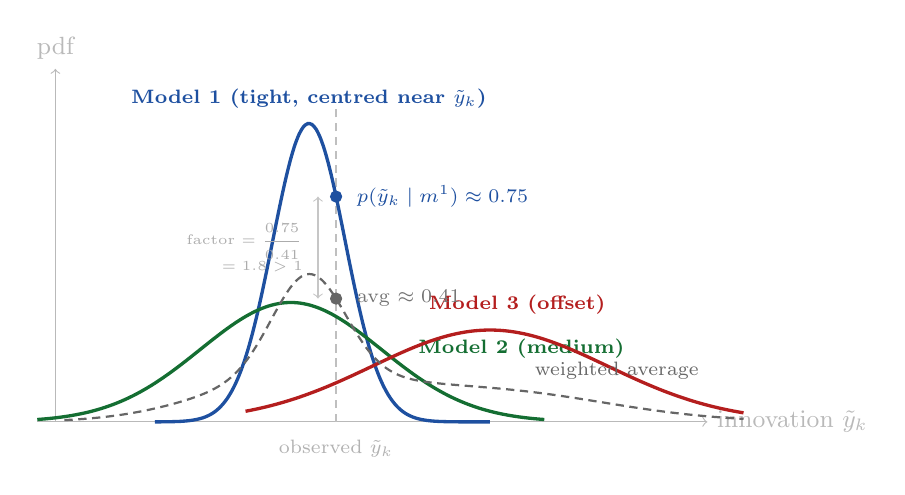
\begin{tikzpicture}[x=1.15cm, y=3.8cm]

  % ── Axes ──────────────────────────────────────────────────────────────────
  \draw[->, gray!55] (-2.8, 0) -- (4.6, 0)
    node[right, font=\small] {innovation $\tilde{y}_k$};
  \draw[->, gray!55] (-2.6, 0) -- (-2.6, 1.18)
    node[above, font=\small] {pdf};

  % ── Vertical line at observed innovation ──────────────────────────────────
  \draw[densely dashed, gray!50, thick] (0.5, 0) -- (0.5, 1.06);
  \node[below=3pt, font=\scriptsize, color=gray!60] at (0.5, 0)
    {observed $\tilde{y}_k$};

  % ── Model 1: tight N(0.2, 0.4²), peak ≈ 1.00 ─────────────────────────────
  \draw[very thick, color=keyblue, domain=-1.5:2.2, samples=80, smooth]
    plot (\x, {exp(-(\x-0.2)*(\x-0.2)/0.32)/(0.4*2.5066)});
  \node[above=2pt, font=\scriptsize\bfseries, color=keyblue] at (0.2, 0.997)
    {Model 1 (tight, centred near $\tilde{y}_k$)};

  % ── Model 2: medium N(0, 1.0), peak ≈ 0.40 ───────────────────────────────
  \draw[very thick, color=defgreen, domain=-2.8:2.8, samples=80, smooth]
    plot (\x, {exp(-\x*\x/2)/2.5066});
  \node[below right, font=\scriptsize\bfseries, color=defgreen] at (1.3, 0.31)
    {Model 2 (medium)};

  % ── Model 3: offset N(2.2, 1.3²), peak ≈ 0.31 ────────────────────────────
  \draw[very thick, color=warnred, domain=-0.5:5.0, samples=80, smooth]
    plot (\x, {exp(-(\x-2.2)*(\x-2.2)/3.38)/3.258});
  \node[above=2pt, font=\scriptsize\bfseries, color=warnred] at (2.5, 0.307)
    {Model 3 (offset)};

  % ── Weighted average ──────────────────────────────────────────────────────
  \draw[thick, densely dashed, color=black!60,
        domain=-2.5:5.0, samples=130, smooth]
    plot (\x, {( exp(-(\x-0.2)*(\x-0.2)/0.32)/(0.4*2.5066)
              + exp(-\x*\x/2)/2.5066
              + exp(-(\x-2.2)*(\x-2.2)/3.38)/3.258
              )/3});
  \node[font=\scriptsize, color=black!60] at (3.6, 0.17)
    {weighted average};

  % ── Dots at the observation x = 0.5 ─────────────────────────────────────
  % Model 1: ≈ 0.753
  \filldraw[keyblue] (0.5, 0.753) circle (2.0pt);
  \node[right=4pt, font=\scriptsize, color=keyblue] at (0.5, 0.753)
    {$p(\tilde{y}_k\mid m^1)\approx 0.75$};
  % Average: ≈ 0.412
  \filldraw[black!60] (0.5, 0.412) circle (2.0pt);
  \node[right=4pt, font=\scriptsize, color=black!55] at (0.5, 0.412)
    {avg $\approx 0.41$};

  % ── Arrow between the two dots ───────────────────────────────────────────
  \draw[<->, thin, gray!45] (0.3, 0.412) -- (0.3, 0.753)
    node[midway, left=2pt, font=\tiny, color=gray!65, align=right]
      {factor $= \dfrac{0.75}{0.41}$\\$= 1.8 > 1$};

\end{tikzpicture}
\caption{
  Each model predicts the innovation will follow its own Gaussian curve.
  $p(\tilde{y}_k \mid m^j)$ is simply the \textbf{height of that curve
  at the point where the actual innovation landed} (vertical dashed line).
  The dashed black curve is the weighted average of all three ---
  the denominator of the Bayes update.
  Model~1's tight Gaussian reads off a higher value than the average at
  this observation point, so its update factor exceeds~1 and its
  probability increases.
  \textit{Note:} if the observation had landed far to the right (e.g.\
  at $\tilde{y}_k = 3$), Model~1's narrow curve would give nearly zero
  there while Model~3's wide curve remains non-negligible --- tight is
  only an advantage when the model is correct.}
\end{figure}

% ------------------------------------------------------------------------------
\subsection*{3.4 \quad Fused State Estimate and Covariance}
% ------------------------------------------------------------------------------

\begin{figure}[H]
  \centering
  
\includegraphics[width=0.82\textwidth]{slide-12.jpg}
  \caption{Calculation of the fused state estimate $\hat{x}_{k|k}$ as a
    probability-weighted average of all model-specific KF estimates.}
\end{figure}

Each of the $J$ Kalman filters produces its own state estimate
$\hat{x}_{k|k}^j$.
The overall fused estimate is the \textbf{probability-weighted average}
over all models, using the \emph{law of total expectation}:
\[
  \hat{x}_{k|k}
  = \mathrm{E}(x_k \mid \mathcal{Y}_k)
  = \sum_{j=1}^{J} p(m^j \mid \mathcal{Y}_k)\;\hat{x}_{k|k}^j
\]
If one model has probability near 1, the fused estimate is almost entirely
that model's estimate.
If two models are equally probable, the fused estimate sits between them.

\begin{figure}[H]
  \centering
  
\includegraphics[width=0.82\textwidth]{slide-13.jpg}
  \caption{Calculation of the fused covariance $P_{k|k}$.
    The total covariance has two contributions: the weighted average of
    each model's own KF covariance, plus the spread of model-specific
    estimates around the fused estimate.}
\end{figure}

The fused covariance uses the \textbf{law of total variance}:
\[
  P_{k|k}
  = \mathrm{V}(x_k \mid \mathcal{Y}_k)
  = \sum_{j=1}^{J} p(m^j \mid \mathcal{Y}_k)
    \Bigl[
      P_{k|k}^j
      + \bigl(\hat{x}_{k|k}^j - \hat{x}_{k|k}\bigr)
        \bigl(\hat{x}_{k|k}^j - \hat{x}_{k|k}\bigr)^\top
    \Bigr]
\]

\begin{center}
\begin{tabular}{@{} l p{3.2cm} p{7.2cm} @{}}
  \toprule
  Symbol & Name & Meaning \\
  \midrule
  $\hat{x}_{k|k}^j$ & Model-$j$ state estimate &
    The KF estimate of the state at time $k$ given all data up to $k$,
    using model $j$. \\
  $P_{k|k}^j$ & Model-$j$ state error covariance &
    The covariance of the error between the KF state estimate and the
    true state, assuming model $j$ is correct:
    $E[(x_k - \hat{x}_{k|k}^j)(x_k - \hat{x}_{k|k}^j)^\top]$.
    This is exactly the standard KF covariance matrix --- the same
    $P_{k|k}$ computed in every Kalman filter predict-update step ---
    just one copy per model.
    Its diagonal entries are the variances of each state component
    (how far off the $x$, $y$, velocity estimates etc.\ could be);
    off-diagonals are correlations between state errors. \\
  $\hat{x}_{k|k}$ & Fused estimate &
    The probability-weighted average across all models. \\
  $P_{k|k}$ & Fused covariance &
    Total uncertainty including both within-model uncertainty and
    between-model disagreement. \\
  \bottomrule
\end{tabular}
\end{center}

\begin{notebox}
  \textbf{Why the fused covariance has an extra term}

  The total uncertainty in the state has two independent sources:

  \textbf{1.\ Within-model uncertainty} $P_{k|k}^j$: suppose you already
  knew for certain that model $j$ was the correct one.
  Even then, the KF estimate $\hat{x}_{k|k}^j$ would still have error ---
  because measurements are noisy, the filter may not have fully converged
  yet, or the process noise keeps the state uncertain.
  $P_{k|k}^j$ is the KF's own estimate of this irreducible uncertainty.
  The models may all agree closely on the state (small second term), but
  if each individual KF is itself uncertain about where the state is
  (large $P_{k|k}^j$), the total uncertainty is still large.
  The weighted average $\sum_j p(m^j|\mathcal{Y}_k)\,P_{k|k}^j$ captures
  this baseline estimation uncertainty.

  \textbf{2.\ Between-model disagreement}
  $(\hat{x}_{k|k}^j - \hat{x}_{k|k})(\hat{x}_{k|k}^j -
  \hat{x}_{k|k})^\top$: different models give different state estimates.
  The fused covariance must account for the fact that we are not certain
  \emph{which} estimate to trust.
  Even if each individual KF is very confident (small $P^j$), if the
  models disagree on where the state is, the overall uncertainty is large.

  Concretely: imagine two models --- one estimates position as 5\,m, the
  other as 10\,m, each with only 0.1\,m uncertainty.
  The fused estimate might be 7.5\,m, but the true uncertainty is not
  0.1\,m --- it is driven by the 5\,m gap between the models.
  The second term captures exactly that spread.
\end{notebox}

% ------------------------------------------------------------------------------
\subsection*{3.5 \quad Computing the Likelihood $p(\tilde{y}_k \mid m^j)$}
% ------------------------------------------------------------------------------

\begin{figure}[H]
  \centering
  
\includegraphics[width=0.82\textwidth]{slide-14.jpg}
  \caption{The likelihood $p(\tilde{y}_k \mid m^j)$ is the Gaussian pdf
    of the KF innovation for model $j$, evaluated at the observed
    innovation value.}
\end{figure}

The Bayes update in Section~3.3 requires $p(\tilde{y}_k \mid m^j)$ ---
the probability of observing the current innovation under model $j$.
This comes directly from the Kalman filter for model $j$.

The innovation for model $j$ is:
\[
  \tilde{y}_k \mid m^j
  \;\triangleq\; y_k - \mathrm{E}(y_k \mid \mathcal{Y}_{k-1},\, m^j)
\]
which is simply the output prediction error of the KF running with model
$j$ --- exactly the same residual used in model validation (Section~2).

Under the Gaussian and linearity assumptions the innovation is normally
distributed:
\[
  p(\tilde{y}_k \mid m^j)
  = \frac{1}{(2\pi)^{n/2}\,|P_k^{yj}|^{1/2}}\;
    \exp\!\left(-\tfrac{1}{2}\,
      \tilde{y}_k^\top (P_k^{yj})^{-1} \tilde{y}_k
    \right)
\]
where $n = \dim(y)$ and $P_k^{yj}$ is the innovation covariance for
model $j$:
\[
  P_k^{yj} = H P_{k|k-1}^j H^\top + R_k
\]

\begin{center}
\begin{tabular}{@{} l p{3.0cm} p{7.4cm} @{}}
  \toprule
  Symbol & Name & Meaning \\
  \midrule
  $\tilde{y}_k \mid m^j$ & Innovation for model $j$ &
    The difference between the actual measurement $y_k$ and what model
    $j$'s KF predicted.
    A large innovation means model $j$ was surprised by the measurement
    --- it fits the data poorly. \\
  $P_k^{yj}$ & Innovation covariance &
    The covariance matrix of the innovation under model $j$ --- it
    defines the exact shape of the Gaussian that $\tilde{y}_k$ is
    expected to follow.
    The diagonal entries are the variances of each output variable
    (how much each is expected to fluctuate); the off-diagonal entries
    are the correlations between output variables.
    \emph{Large values on the diagonal} of $P_k^{yj}$ mean large
    variances --- model $j$ has wide spread and is not very certain what
    it will observe, so even a large innovation is not that surprising
    and does not penalise the model much.
    \emph{Small values on the diagonal} mean small variances --- model
    $j$ is confident in its prediction, so a large innovation is very
    unlikely under this model and penalises it heavily.
    It is computed as $P_k^{yj} = HP_{k|k-1}^j H^\top + R_k$: the
    state estimation uncertainty mapped to output space, plus the
    measurement noise. \\
  $H$ & Observation matrix & Maps the state to the measurement space. \\
  $P_{k|k-1}^j$ & Predicted state covariance &
    Model $j$'s uncertainty in the predicted state before the measurement
    update. \\
  $R_k$ & Measurement noise covariance & Noise on the sensor itself. \\
  \bottomrule
\end{tabular}
\end{center}

\begin{notebox}
  \textbf{What this probability actually measures}

  $p(\tilde{y}_k \mid m^j)$ is high when the observed innovation
  $\tilde{y}_k$ is small relative to $P_k^{yj}$ --- model $j$ predicted
  the measurement accurately and was not surprised.

  $p(\tilde{y}_k \mid m^j)$ is low when $\tilde{y}_k$ is large relative
  to $P_k^{yj}$ --- the actual measurement was far from what model $j$
  expected.

  This is precisely what drives the probability update: models that are
  consistently ``surprised'' by the data have their probability driven
  toward zero, while models that consistently predict well are driven
  toward one.
  Every KF already computes both $\tilde{y}_k^j$ and $P_k^{yj}$ as
  part of its normal operation --- the multi-model extension requires no
  extra computation beyond evaluating the Gaussian pdf at the existing
  innovation.
\end{notebox}

% ------------------------------------------------------------------------------
\subsection*{3.6 \quad Block Diagram --- Putting It All Together}
% ------------------------------------------------------------------------------

\begin{figure}[H]
  \centering
  
\includegraphics[width=0.88\textwidth]{slide-15.jpg}
  \caption{Block diagram of the multi-model filter (static case).
    $J$ parallel Kalman filters each process the same measurement $y_k$.
    Their innovations feed a model probability block that updates
    $\{p(m^j|\mathcal{Y}_k)\}$.
    The fused state estimate and covariance are computed from the
    probability-weighted combination of all KF outputs.}
\end{figure}

The complete filter runs as follows at each time step $k$:

\begin{enumerate}[leftmargin=1.5em, itemsep=8pt]

  \item \textbf{Run all $J$ Kalman filters independently.}
    Every filter sees the same new measurement $y_k$ but uses its own
    model matrices $\Phi^j$, $H^j$, $Q^j$.
    Each runs a standard predict-update cycle to produce the four
    outputs needed by the later steps:
    \begin{align*}
      \hat{x}_{k|k-1}^j &= \Phi^j\,\hat{x}_{k-1|k-1}^j
        & &\text{(predicted state)} \\
      P_{k|k-1}^j &= \Phi^j P_{k-1|k-1}^j (\Phi^j)^\top + Q^j
        & &\text{(predicted covariance)} \\
      \tilde{y}_k^j &= y_k - H^j\hat{x}_{k|k-1}^j
        & &\text{(innovation --- how surprised model $j$ is)} \\
      P_k^{yj} &= H^j P_{k|k-1}^j (H^j)^\top + R_k
        & &\text{(innovation covariance)} \\
      K_k^j &= P_{k|k-1}^j (H^j)^\top (P_k^{yj})^{-1}
        & &\text{(Kalman gain)} \\
      \hat{x}_{k|k}^j &= \hat{x}_{k|k-1}^j + K_k^j\,\tilde{y}_k^j
        & &\text{(updated state estimate)} \\
      P_{k|k}^j &= (I - K_k^j H^j)\,P_{k|k-1}^j
        & &\text{(updated state covariance)}
    \end{align*}
    The key outputs passed to the next steps are:
    $\tilde{y}_k^j$ (innovation),
    $P_k^{yj}$ (innovation covariance),
    $\hat{x}_{k|k}^j$ (updated state estimate), and
    $P_{k|k}^j$ (updated state error covariance).

  \item \textbf{Use the innovation $\tilde{y}_k^j$ and innovation
    covariance $P_k^{yj}$ from step~1 to compute each model's
    likelihood.}
    This is the height of model $j$'s Gaussian pdf evaluated at the
    observed innovation --- how well model $j$ predicted what just
    happened:
    \[
      p(\tilde{y}_k \mid m^j)
      = \frac{1}{(2\pi)^{n/2}|P_k^{yj}|^{1/2}}
        \exp\!\left(
          -\tfrac{1}{2}\,\tilde{y}_k^\top (P_k^{yj})^{-1}\tilde{y}_k
        \right), \quad n = \dim(y_k)
    \]
    These $J$ likelihood values $p(\tilde{y}_k \mid m^j)$ feed directly
    into step~3.

  \item \textbf{Use the likelihoods $p(\tilde{y}_k \mid m^j)$ from
    step~2 and the previous model probabilities
    $p(m^j \mid \mathcal{Y}_{k-1})$ to update the model probabilities
    via Bayes:}
    \[
      p(m^j \mid \mathcal{Y}_k)
      = \frac{p(\tilde{y}_k \mid m^j)\;p(m^j \mid \mathcal{Y}_{k-1})}
             {\displaystyle\sum_{l=1}^{J}
              p(\tilde{y}_k \mid m^l)\;p(m^l \mid \mathcal{Y}_{k-1})}
    \]
    Models that predicted well gain probability; those that predicted
    poorly lose it.
    The updated model probabilities $p(m^j \mid \mathcal{Y}_k)$ feed
    directly into step~4.

  \item \textbf{Use the updated model probabilities
    $p(m^j \mid \mathcal{Y}_k)$ from step~3 together with the updated
    state estimates $\hat{x}_{k|k}^j$ and state error covariances
    $P_{k|k}^j$ from step~1 to fuse into the final output:}
    \[
      \hat{x}_{k|k}
      = \sum_{j=1}^{J} p(m^j \mid \mathcal{Y}_k)\;\hat{x}_{k|k}^j
      \quad \text{(fused state estimate)}
    \]
    \[
      P_{k|k}
      = \sum_{j=1}^{J} p(m^j \mid \mathcal{Y}_k)
        \Bigl[
          P_{k|k}^j
          + \bigl(\hat{x}_{k|k}^j - \hat{x}_{k|k}\bigr)
            \bigl(\hat{x}_{k|k}^j - \hat{x}_{k|k}\bigr)^\top
        \Bigr]
      \quad \text{(fused state error covariance)}
    \]
    The outputs --- fused state estimate $\hat{x}_{k|k}$, fused
    covariance $P_{k|k}$, and updated model probabilities
    $p(m^j \mid \mathcal{Y}_k)$ --- become the inputs for the next
    time step $k{+}1$.

\end{enumerate}

The ``Residual'' boxes in the block diagram compute
$\tilde{y}_{k|k-1}^l = y_k - \hat{y}_{k|k-1}^l$ and pass the result to
the model probability block alongside $P_{y,k|k-1}^l$.
Note that the residual block does \emph{not} need the full KF update ---
it only needs the prediction step output to form the innovation.

% ------------------------------------------------------------------------------
\subsection*{3.7 \quad Adaptive Case --- Models Changing with Time}
% ------------------------------------------------------------------------------

\begin{figure}[H]
  \centering
  
\includegraphics[width=0.78\textwidth]{slide-16.jpg}
  \caption{In the adaptive case the correct model may switch between
    time steps.
    Two approaches: floor the static-case probabilities to keep all
    filters alive, or model switching explicitly using Markov chains.}
\end{figure}

The static case assumes one model is correct forever.
In hybrid systems --- where the true model can switch (e.g.\ a vehicle
transitioning from dry to icy road) --- the static filter eventually
kills off all but one model and cannot recover when the switch occurs.

\textbf{Approach 1 --- Probability flooring (simple):}
Run the static update, but after each step \emph{clip} the model
probabilities to a minimum value significantly less than $1/J$:
\[
  p(m^j \mid \mathcal{Y}_k) \;\geq\; p_{\min}
  \quad\text{(e.g.\ } p_{\min} = 0.01 \text{ for } J = 3\text{)}
\]
\begin{notebox}
  \textbf{What flooring does --- and what it does not do}

  The goal is \emph{not} to keep all probabilities low.
  One model is still allowed to dominate and be close to~1.
  The floor is purely a safety net for the \emph{other} models ---
  it prevents any single model from reaching exactly zero and dying.

  Without the floor: once a model's probability drops very close to
  zero, its KF gets negligible weight in the fused estimate and its
  innovations stop influencing the probability update.
  It is effectively dead.
  If the correct model later switches to that dead model, it cannot
  recover quickly because it has been starved of weight for many steps
  and needs many new measurements to climb back up.

  With the floor: all KFs always receive at least a small weight.
  They keep running, their innovations keep being computed, and if their
  model becomes correct again they can rapidly climb back to dominance.
  The trade-off: the dominant model can never quite reach probability 1,
  but in a switching system this is the right choice.
\end{notebox}

\textbf{Approach 2 --- Markov chain model (more accurate):}
Introduce a \textbf{transition matrix} $\Pi$ where entry $\Pi_{jl}$
is the probability that the correct model switches \emph{from} model
$l$ \emph{to} model $j$ in one time step.

\begin{notebox}
  \textbf{What the Markov chain changes --- and what it does not}

  The individual Kalman filters are \emph{not} modified.
  All $J$ KFs continue running with their fixed model parameters
  $\Phi^j$, $H^j$, $Q^j$ throughout.
  The KF itself does not detect any switch.

  What changes is only the \textbf{probability prediction step}.
  In the static case, before a new measurement arrives, the model
  probabilities are simply carried forward unchanged.
  With the Markov chain, the probabilities are first
  \emph{predicted forward} using the transition matrix:
  \[
    p_{\text{pred}}(m^j \mid \mathcal{Y}_{k-1})
    = \sum_{l=1}^{J} \Pi_{jl}\;p(m^l \mid \mathcal{Y}_{k-1})
  \]
  This allows some probability to ``bleed'' from every model to every
  other model before the measurement update, so no model ever collapses
  to zero on its own.
  The Bayes update (step~3 in Section~3.6) then runs as usual using
  these predicted probabilities.

  In practice the transition matrix $\Pi$ needs to be designed by the
  user to reflect how fast and how often the true model is expected to
  switch --- which is often unknown, making approximate methods
  necessary.
\end{notebox}

% ── Key takeaways ─────────────────────────────────────────────────────────────
\begin{keybox}
  \textbf{Section 3 --- Key Takeaways}
  \begin{itemize}[leftmargin=1.2em, itemsep=2pt]
    \item Run $J$ parallel Kalman filters, one per candidate model.
      Track the \textbf{posterior probability} $p(m^j|\mathcal{Y}_k)$ of
      each model being correct.
    \item Probabilities are updated by Bayes' rule:
      $p(m^j|\mathcal{Y}_k) \propto p(\tilde{y}_k|m^j) \cdot
      p(m^j|\mathcal{Y}_{k-1})$.
      Models that predict measurements well gain probability; those that
      predict poorly lose it.
      Over time the true model converges to probability~1.
    \item The likelihood $p(\tilde{y}_k|m^j)$ is the Gaussian pdf of
      the KF innovation --- already computed as part of normal KF
      operation.
    \item Fused estimate:
      $\hat{x}_{k|k} = \sum_j p(m^j|\mathcal{Y}_k)\,\hat{x}_{k|k}^j$.
      Fused covariance adds a \textbf{between-model spread term} on top
      of each model's own KF covariance.
    \item \textbf{Static case:} one model stays correct forever.
      \textbf{Adaptive case:} floor probabilities to keep all filters
      alive when models can switch.
  \end{itemize}
\end{keybox}

% ==============================================================================
\clearpage
\section*{Section 4 \quad Parameter Estimation}
% ==============================================================================

Section~3 handled model uncertainty by choosing between a small discrete
set of candidate models.
Section~4 handles a different situation: you have \textbf{one model
structure} that you believe is correct, but some of its numerical
parameters are unknown, poorly known, or slowly changing over time.

Rather than picking between fixed alternatives, the goal here is to
\textbf{estimate the parameter values directly from data}.

% ------------------------------------------------------------------------------
\subsection*{4.1 \quad Overview --- When Parameters Need Estimating}
% ------------------------------------------------------------------------------

\begin{figure}[H]
  \centering
  
\includegraphics[width=0.78\textwidth]{slide-17.jpg}
  \caption{Two main approaches to parameter estimation: augmenting the
    state vector and using EKF/UKF, or using system identification
    methods based on maximum likelihood.}
\end{figure}

If the model structure is correct but a parameter vector $\theta$ is
unknown or drifting slowly, there are two main strategies:

\begin{itemize}[leftmargin=1.5em, itemsep=4pt]
  \item \textbf{Include $\theta$ as extra states and use EKF/UKF.}
    Augment the state vector with the unknown parameters and run an
    extended or unscented Kalman filter that estimates both the physical
    states and the parameters simultaneously, online in real time.
    Covered in Section~4.2.

  \item \textbf{System identification (SI) --- maximum likelihood.}
    Treat the parameters as fixed unknowns and find the values that make
    the observed data most probable.
    This is done offline (using a collected dataset) and gives a single
    best-fit parameter set rather than a time-varying estimate.
    Covered in Sections~4.3--4.4.
\end{itemize}

% ------------------------------------------------------------------------------
\subsection*{4.2 \quad Method 1 --- Parameters as Augmented States}
% ------------------------------------------------------------------------------

\begin{figure}[H]
  \centering
  
\includegraphics[width=0.78\textwidth]{slide-18.jpg}
  \caption{The parameter vector $\theta$ is given its own state-space
    model $\theta_{k+1} = A\theta_k + \nu_k$ and appended to the
    physical state, allowing joint estimation of states and parameters.}
\end{figure}

The idea is to append the unknown parameter vector $\theta$ to the
physical state vector and then run a filter on the combined system.
The parameter dynamics are described by an additional state model:
\[
  \theta_{k+1} = A\,\theta_k + \nu_k,
  \qquad \nu_k \in \mathrm{NID}(\mathbf{0},\,\Sigma),
  \qquad \mathrm{Cov}(\theta_0) = \Pi
\]

The matrices $A$, $\Sigma$, and $\Pi$ are chosen by the user to describe
how the parameter is expected to behave:

\begin{center}
\begin{tabular}{@{} l p{3.5cm} p{7.0cm} @{}}
  \toprule
  Choice & Behaviour & Physical meaning \\
  \midrule
  $A = I,\;\Sigma = 0,\;\Pi > 0$ & Unknown but constant &
    The parameter is fixed and unknown.
    The filter estimates it once and does not let it drift.
    The initial covariance $\Pi$ reflects how uncertain you are about
    its value at the start. \\[4pt]
  $A = I,\;\Sigma > 0,\;\Pi > 0$ & Slowly varying, unbounded &
    The parameter is allowed to drift in a random walk.
    It can end up anywhere over time.
    Use when you know the parameter changes but have no idea about its
    long-run value (e.g.\ a slowly corroding component). \\[4pt]
  $A < I,\;\Sigma > 0,\;\Pi > 0$ & Slowly varying, bounded range &
    $A < I$ introduces a restoring force toward zero, so the parameter
    wanders but stays within a limited range.
    Use when you believe the parameter varies but cannot drift
    arbitrarily (e.g.\ a temperature-dependent coefficient that stays
    within physical limits). \\
  \bottomrule
\end{tabular}
\end{center}

\begin{notebox}
  \textbf{Why EKF or UKF --- not the regular KF?}

  Once $\theta$ is appended to the state, the combined state vector is
  $[x^\top,\;\theta^\top]^\top$.
  The original system equations typically involve $\theta$
  \emph{multiplied by} state variables --- for example,
  $\dot{x} = A(\theta)\,x$.
  This product makes the combined dynamics \textbf{nonlinear} in the
  augmented state, even if the original system was linear in $x$ alone.

  A standard Kalman filter cannot handle this.
  The \textbf{EKF} linearises the combined dynamics at the current
  estimate using a Jacobian; the \textbf{UKF} propagates a set of
  sigma points through the exact nonlinear equations.
  Both can track slowly varying parameters --- how well depends on
  how nonlinear the coupling is and how fast the parameter changes
  relative to the sampling rate.
\end{notebox}

% ------------------------------------------------------------------------------
\subsection*{4.3 \quad Method 2 --- Maximum Likelihood Estimation}
% ------------------------------------------------------------------------------

\begin{figure}[H]
  \centering
  
\includegraphics[width=0.78\textwidth]{slide-17.jpg}
  \caption{Maximum likelihood: find the parameter vector $\theta$ that
    maximises the probability of observing the collected dataset.}
\end{figure}

If the parameters are \emph{fixed} (not time-varying), a cleaner
offline approach is \textbf{maximum likelihood (ML)} estimation.
Given a dataset $\mathcal{Y}_N = \{y_1,\ldots,y_N\}$, the ML estimate is:
\[
  \hat{\theta}_{ML}
  = \arg\max_{\theta}\; L(\theta),
  \qquad L(\theta) = p(\mathcal{Y}_N,\,\theta)
\]

\begin{center}
\begin{tabular}{@{} l p{3.0cm} p{7.5cm} @{}}
  \toprule
  Symbol & Name & Meaning \\
  \midrule
  $\theta$ & Parameter vector &
    The unknown model parameters to be estimated (e.g.\ damping
    coefficient, time constant, sensor gain). \\
  $L(\theta)$ & Likelihood function &
    The probability of observing the entire dataset $\mathcal{Y}_N$
    given a specific choice of $\theta$.
    High $L$ means $\theta$ fits the data well; low $L$ means it does
    not. \\
  $\hat{\theta}_{ML}$ & ML estimate &
    The value of $\theta$ that makes the observed data most probable ---
    the best-fitting parameter set. \\
  \bottomrule
\end{tabular}
\end{center}

\begin{notebox}
  \textbf{What maximising the likelihood means in plain terms}

  Method~2 does still use a Kalman filter, but in a completely different
  role to Method~1.

  In \textbf{Method~1} (augmented state), the KF \emph{estimates}
  $\theta$ directly --- $\theta$ is part of the state vector and the
  filter updates it every step.

  In \textbf{Method~2} (ML), the KF is only used as an
  \emph{evaluation tool} inside an outer optimisation loop.
  You fix $\theta$ at some trial value, run a standard KF (no
  augmentation), and compute the innovations $\tilde{y}_{k|k-1}$.
  Those innovations tell you how surprised the model was by the data
  under that particular $\theta$.
  If $\theta$ is correct, the innovations should be white noise with
  covariance $P_k^y$.
  The likelihood $L(\theta)$ measures exactly how well they match that
  expectation.

  The outer optimiser (e.g.\ gradient ascent, Nelder-Mead) then tries
  a new $\theta$, runs the KF again, computes $L$ again, and repeats
  until it finds the $\theta$ that makes the innovations look most like
  white noise.
  That is the ML estimate.
  The KF never estimates $\theta$ --- the optimiser does, by searching
  over the space of possible values.
\end{notebox}

% ------------------------------------------------------------------------------
\subsection*{4.4 \quad System Identification Methods --- Taxonomy}
% ------------------------------------------------------------------------------

\begin{figure}[H]
  \centering
  
\includegraphics[width=0.78\textwidth]{slide-19.jpg}
  \caption{Overview of system identification method families.
    The choice of method depends on model structure (black box vs grey
    box), linearity, and whether the system is modelled in discrete or
    continuous time.}
\end{figure}

System identification (SI) covers a broad family of methods for fitting
model parameters to data.
The choice of method depends on what you know about the model structure:

\textbf{Discrete-time, linear:}
\begin{itemize}[leftmargin=1.5em, itemsep=2pt]
  \item \emph{Black box} --- you have no physical model; estimate all
    parameters of a general ARX/ARMAX/state-space structure with no
    particular physical meaning.
    Methods: prediction error methods (PEM), subspace methods.
  \item \emph{Grey box} --- you have a physical model with known
    structure but unknown parameter values.
    Methods: prediction error methods, maximum likelihood.
\end{itemize}

\textbf{Discrete-time, nonlinear:}
Mostly grey box models since a black-box nonlinear parameterisation
would require an enormous number of parameters.

\textbf{Continuous-time:}
Mostly grey box for linear and mildly nonlinear systems.
The likelihood function is evaluated using the \textbf{continuous-discrete
Kalman filter (CD-KF)}, which handles systems specified with continuous
dynamics $\dot{x} = f(x,\theta) + w$ but discrete measurements.
The CD-KF computes the innovations and their covariances in the same way
as the standard KF --- the only difference is how the state is propagated
between measurement steps (using continuous-time integration rather than
a discrete matrix multiply).
The likelihood is then assembled from those innovations exactly as in
Section~4.5 below.

% ------------------------------------------------------------------------------
\subsection*{4.5 \quad Computing the Likelihood via KF Innovations}
% ------------------------------------------------------------------------------

\begin{figure}[H]
  \centering
  
\includegraphics[width=0.78\textwidth]{slide-20.jpg}
  \caption{The likelihood factorises into a product of Gaussian pdfs of
    the KF innovations, one per time step, with innovation covariance
    $P_k^y = HP_{k|k-1}H^\top + R_k$.
    This formula applies to both discrete-time and continuous-time
    (CD-KF) systems.}
\end{figure}

For both discrete-time and continuous-time systems, the likelihood
factorises into a product over time steps:
\[
  L(\theta)
  = p(\mathcal{Y}_N \mid \theta)
  = \prod_{k=1}^{N} p\!\bigl(\tilde{y}_{k|k-1} \mid \theta\bigr)
\]
Each factor is the Gaussian pdf of the innovation at step $k$:
\[
  p(\tilde{y}_{k|k-1})
  = \frac{1}{(2\pi)^{n/2}\,|P_k^y|^{1/2}}\;
    \exp\!\left(
      -\tfrac{1}{2}\,\tilde{y}_{k|k-1}^\top\,(P_k^y)^{-1}\,\tilde{y}_{k|k-1}
    \right),
  \quad n = \dim(y)
\]
where $P_k^y = H P_{k|k-1} H^\top + R_k$ is the innovation covariance.

\begin{notebox}
  \textbf{Why the likelihood factorises into a product of innovations}

  This follows from the fact that given the model and all previous
  measurements, the next innovation is conditionally independent of
  the ones before it.
  Each innovation carries one step's worth of ``new information'' about
  the data.
  Taking the product over all $N$ steps gives the total probability of
  having seen the entire sequence.

  In practice it is more numerically stable to work with the
  \textbf{log-likelihood}:
  \[
    \ln L(\theta)
    = -\frac{1}{2}\sum_{k=1}^{N}
      \Bigl[
        n\ln(2\pi)
        + \ln|P_k^y|
        + \tilde{y}_{k|k-1}^\top\,(P_k^y)^{-1}\,\tilde{y}_{k|k-1}
      \Bigr]
  \]
  The product becomes a sum, which avoids underflow when multiplying
  many small probabilities together.
  Maximising $\ln L$ is equivalent to maximising $L$ since $\ln$ is
  monotone.
\end{notebox}

\begin{notebox}
  \textbf{Black box vs grey box --- the key distinction}

  A \textbf{black-box} model makes no assumptions about the physical
  process.
  It fits a general mathematical structure (polynomial, rational
  function, neural network) purely to reproduce the input-output
  behaviour.
  This requires many parameters and gives no physical insight.

  A \textbf{grey-box} model starts from the physical equations of motion
  (derived from Newton's laws, circuit theory, thermodynamics, etc.) and
  only estimates the unknown numerical coefficients (masses, damping
  ratios, time constants).
  Far fewer parameters need to be estimated, the estimates have direct
  physical meaning, and the model generalises better outside the
  training data.
  For engineering applications where a physical model exists, grey-box
  identification is almost always preferable.

  \textbf{Practical advice:} start by estimating as few parameters as
  possible.
  Each additional unknown parameter makes the optimisation harder and
  increases the risk of finding a local maximum of $L(\theta)$ that
  does not represent the true physical values.
\end{notebox}

% ── Key takeaways ─────────────────────────────────────────────────────────────
\begin{keybox}
  \textbf{Section 4 --- Key Takeaways}
  \begin{itemize}[leftmargin=1.2em, itemsep=2pt]
    \item Parameter estimation addresses a different problem than
      multi-model estimation: one model structure, unknown continuous
      parameter values rather than a discrete set of candidates.
    \item \textbf{Method 1 --- augmented state:} append $\theta$ to the
      state vector with dynamics $\theta_{k+1} = A\theta_k + \nu_k$.
      Choose $A$, $\Sigma$, $\Pi$ to reflect whether $\theta$ is
      constant ($\Sigma = 0$), a random walk ($A = I$), or mean-reverting
      ($A < I$).
      EKF or UKF required because $\theta$ enters the dynamics
      nonlinearly.
    \item \textbf{Method 2 --- maximum likelihood:}
      $\hat{\theta}_{ML} = \arg\max_\theta\,p(\mathcal{Y}_N,\theta)$.
      Run the KF for each candidate $\theta$ and evaluate
      $L(\theta) = \prod_k p(\tilde{y}_{k|k-1})$ --- the product of
      Gaussian innovation pdfs.
      Use log-likelihood in practice to avoid numerical underflow.
    \item Black-box SI estimates all parameters with no physical
      structure; grey-box SI fits unknown coefficients in a
      physically-derived model.
      Grey box is preferred in engineering: fewer parameters, physical
      meaning, better generalisation.
    \item \textbf{Practical rule:} estimate as few parameters as possible
      to avoid local optima and identifiability problems.
  \end{itemize}
\end{keybox}

% ==============================================================================
\clearpage
\section*{Lecture Summary --- Three Approaches to Model Uncertainty}
% ==============================================================================

\begin{keybox}
  \textbf{Approach 1 --- Model Validation (Section~2):
  ``Is the model any good?''}

  This approach does not fix anything --- it \emph{diagnoses}.
  You run the Kalman filter with the model you have and collect the
  residuals (innovations) $\tilde{y}_{k|k-1}$ over a long dataset.
  Then you check whether those residuals have the statistical properties
  they \emph{should} have if the model were correct: zero mean,
  uncorrelated over time (white noise), and Gaussian.

  If the tests pass, you have evidence the model is at least
  statistically consistent with the data.
  If they fail --- residuals are correlated, non-Gaussian, or biased ---
  the model is missing something and can be improved.
  The tests tell you \emph{that} there is a problem; they do not tell
  you \emph{what} to fix.
  Tools: run test (sign changes), ACF / Portmanteau test, normal
  probability plot.
\end{keybox}

\vspace{6pt}

\begin{keybox}
  \textbf{Approach 2 --- Multi-Model Estimation (Section~3):
  ``Which of these candidate models is correct?''}

  This approach is used when you have a small discrete set of candidate
  models --- different suppliers, different parameter values, different
  complexity levels --- and you do not know which is the true one.
  Rather than picking one upfront, you run \emph{all} of them in
  parallel, each as a complete Kalman filter.

  At every time step, you ask each model: how well did you predict the
  measurement that just arrived?
  Models that are consistently surprised (large innovations relative to
  their expected spread) lose probability; models that predict well
  gain probability.
  This is a Bayesian update: the probability of each model being correct
  is updated using the ratio of how well that model fit the new data
  versus the weighted average fit across all models.

  The final state estimate is a probability-weighted blend of all
  model-specific estimates.
  Over time, the true model's probability converges to~1 and the others
  go to~0 --- the data has effectively selected the correct model for
  you.
\end{keybox}

\vspace{6pt}

\begin{keybox}
  \textbf{Approach 3 --- Parameter Estimation (Section~4):
  ``What is the value of this unknown parameter?''}

  This approach is used when the model structure is correct but some
  continuous parameter values are unknown.
  There are two sub-methods:

  \textbf{Online (augmented KF):}
  Append the unknown parameter $\theta$ to the state vector and run an
  EKF or UKF on the combined system.
  The filter estimates both the physical states and $\theta$
  simultaneously at every time step.
  No separate optimisation loop is needed --- the KF does everything.

  \textbf{Offline (maximum likelihood):}
  Here the KF and an optimiser work together in a loop.
  The \emph{optimiser} (e.g.\ gradient ascent, Nelder-Mead) proposes a
  trial value of $\theta$.
  The \emph{KF} is run with that fixed $\theta$ and produces innovations
  $\tilde{y}_{k|k-1}$ --- how surprised the model was at each step.
  The likelihood $L(\theta) = \prod_k p(\tilde{y}_{k|k-1})$ measures
  how well that $\theta$ fits the entire dataset.
  The optimiser uses this score to decide which direction to step next
  --- toward $\theta$ values that make the KF \emph{less} surprised by
  the data (smaller, better-calibrated innovations).
  The KF acts as an indicator of fit quality; the optimiser uses that
  signal to search for the best $\theta$.
  The loop repeats until the likelihood stops improving.
\end{keybox}

\end{document}
